\documentclass{standalone}
\usepackage{tikz}
\begin{document}
% Created by tikzDevice version 0.7.0 on 2015-04-30 12:06:24
% !TEX encoding = UTF-8 Unicode
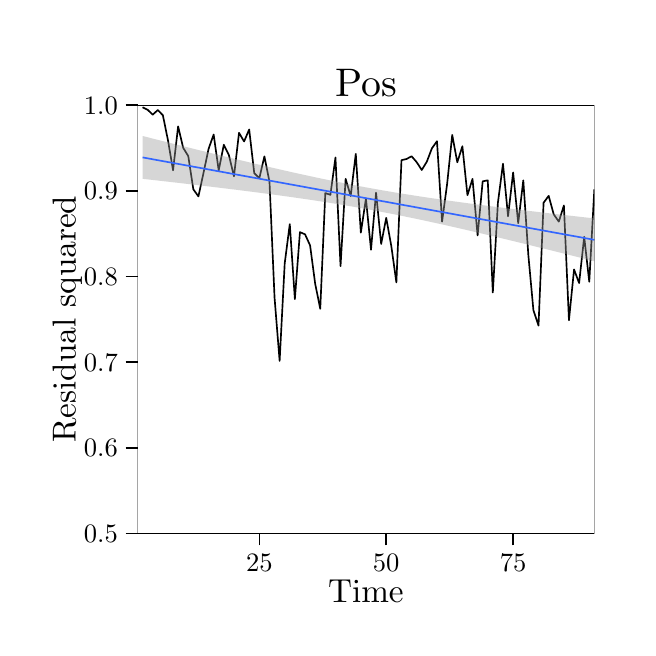
\begin{tikzpicture}[x=1pt,y=1pt]
\definecolor[named]{fillColor}{rgb}{1.00,1.00,1.00}
\path[use as bounding box,fill=fillColor,fill opacity=0.00] (0,0) rectangle (216.81,216.81);
\begin{scope}
\path[clip] (  0.00,  0.00) rectangle (216.81,216.81);
\definecolor[named]{drawColor}{rgb}{1.00,1.00,1.00}
\definecolor[named]{fillColor}{rgb}{1.00,1.00,1.00}

\path[draw=drawColor,line width= 0.6pt,line join=round,line cap=round,fill=fillColor] ( -0.00,  0.00) rectangle (216.81,216.81);
\end{scope}
\begin{scope}
\path[clip] ( 39.69, 34.03) rectangle (204.76,188.82);
\definecolor[named]{fillColor}{rgb}{1.00,1.00,1.00}

\path[fill=fillColor] ( 39.69, 34.03) rectangle (204.76,188.82);
\definecolor[named]{drawColor}{rgb}{0.00,0.00,0.00}

\path[draw=drawColor,line width= 0.6pt,line join=round] ( 41.52,188.04) --
	( 43.35,187.14) --
	( 45.19,185.37) --
	( 47.02,187.05) --
	( 48.86,185.15) --
	( 50.69,176.14) --
	( 52.53,165.27) --
	( 54.36,181.12) --
	( 56.19,173.40) --
	( 58.03,170.40) --
	( 59.86,158.39) --
	( 61.70,155.85) --
	( 63.53,164.30) --
	( 65.37,173.01) --
	( 67.20,178.19) --
	( 69.03,165.21) --
	( 70.87,174.50) --
	( 72.70,170.79) --
	( 74.54,163.11) --
	( 76.37,178.81) --
	( 78.20,175.68) --
	( 80.04,180.03) --
	( 81.87,164.25) --
	( 83.71,162.42) --
	( 85.54,170.29) --
	( 87.38,161.10) --
	( 89.21,119.21) --
	( 91.04, 96.38) --
	( 92.88,131.64) --
	( 94.71,145.82) --
	( 96.55,118.74) --
	( 98.38,142.92) --
	(100.22,142.14) --
	(102.05,138.13) --
	(103.88,124.33) --
	(105.72,115.20) --
	(107.55,157.05) --
	(109.39,156.41) --
	(111.22,169.90) --
	(113.05,130.63) --
	(114.89,162.19) --
	(116.72,155.96) --
	(118.56,171.21) --
	(120.39,142.73) --
	(122.23,155.04) --
	(124.06,136.58) --
	(125.89,157.17) --
	(127.73,138.64) --
	(129.56,148.08) --
	(131.40,137.87) --
	(133.23,124.74) --
	(135.07,168.93) --
	(136.90,169.36) --
	(138.73,170.34) --
	(140.57,168.20) --
	(142.40,165.39) --
	(144.24,168.40) --
	(146.07,173.21) --
	(147.90,175.78) --
	(149.74,146.71) --
	(151.57,160.36) --
	(153.41,178.06) --
	(155.24,168.16) --
	(157.08,173.95) --
	(158.91,156.28) --
	(160.74,162.18) --
	(162.58,141.72) --
	(164.41,161.28) --
	(166.25,161.65) --
	(168.08,121.12) --
	(169.92,153.57) --
	(171.75,167.62) --
	(173.58,148.65) --
	(175.42,164.48) --
	(177.25,146.16) --
	(179.09,161.63) --
	(180.92,134.58) --
	(182.75,114.67) --
	(184.59,109.14) --
	(186.42,153.54) --
	(188.26,156.04) --
	(190.09,149.34) --
	(191.93,146.72) --
	(193.76,152.55) --
	(195.59,111.10) --
	(197.43,129.43) --
	(199.26,124.53) --
	(201.10,141.23) --
	(202.93,124.96) --
	(204.76,158.36);
\definecolor[named]{fillColor}{rgb}{0.60,0.60,0.60}

\path[fill=fillColor,fill opacity=0.40] ( 41.52,177.66) --
	( 43.59,177.14) --
	( 45.65,176.62) --
	( 47.72,176.09) --
	( 49.79,175.58) --
	( 51.85,175.06) --
	( 53.92,174.54) --
	( 55.99,174.02) --
	( 58.05,173.51) --
	( 60.12,173.00) --
	( 62.18,172.49) --
	( 64.25,171.98) --
	( 66.32,171.47) --
	( 68.38,170.96) --
	( 70.45,170.46) --
	( 72.52,169.96) --
	( 74.58,169.46) --
	( 76.65,168.96) --
	( 78.72,168.47) --
	( 80.78,167.98) --
	( 82.85,167.49) --
	( 84.91,167.01) --
	( 86.98,166.53) --
	( 89.05,166.05) --
	( 91.11,165.58) --
	( 93.18,165.11) --
	( 95.25,164.64) --
	( 97.31,164.18) --
	( 99.38,163.73) --
	(101.45,163.28) --
	(103.51,162.83) --
	(105.58,162.39) --
	(107.65,161.96) --
	(109.71,161.54) --
	(111.78,161.12) --
	(113.84,160.70) --
	(115.91,160.30) --
	(117.98,159.90) --
	(120.04,159.51) --
	(122.11,159.12) --
	(124.18,158.75) --
	(126.24,158.38) --
	(128.31,158.01) --
	(130.38,157.66) --
	(132.44,157.31) --
	(134.51,156.97) --
	(136.57,156.64) --
	(138.64,156.31) --
	(140.71,155.99) --
	(142.77,155.67) --
	(144.84,155.36) --
	(146.91,155.06) --
	(148.97,154.76) --
	(151.04,154.46) --
	(153.11,154.17) --
	(155.17,153.89) --
	(157.24,153.61) --
	(159.30,153.33) --
	(161.37,153.06) --
	(163.44,152.79) --
	(165.50,152.52) --
	(167.57,152.26) --
	(169.64,152.00) --
	(171.70,151.74) --
	(173.77,151.49) --
	(175.84,151.24) --
	(177.90,150.99) --
	(179.97,150.74) --
	(182.03,150.49) --
	(184.10,150.25) --
	(186.17,150.00) --
	(188.23,149.76) --
	(190.30,149.52) --
	(192.37,149.28) --
	(194.43,149.05) --
	(196.50,148.81) --
	(198.57,148.58) --
	(200.63,148.34) --
	(202.70,148.11) --
	(204.76,147.88) --
	(204.76,132.41) --
	(202.70,132.93) --
	(200.63,133.45) --
	(198.57,133.98) --
	(196.50,134.49) --
	(194.43,135.01) --
	(192.37,135.53) --
	(190.30,136.05) --
	(188.23,136.56) --
	(186.17,137.07) --
	(184.10,137.58) --
	(182.03,138.09) --
	(179.97,138.60) --
	(177.90,139.11) --
	(175.84,139.61) --
	(173.77,140.11) --
	(171.70,140.61) --
	(169.64,141.11) --
	(167.57,141.60) --
	(165.50,142.09) --
	(163.44,142.58) --
	(161.37,143.06) --
	(159.30,143.54) --
	(157.24,144.02) --
	(155.17,144.49) --
	(153.11,144.96) --
	(151.04,145.43) --
	(148.97,145.89) --
	(146.91,146.34) --
	(144.84,146.79) --
	(142.77,147.24) --
	(140.71,147.67) --
	(138.64,148.11) --
	(136.57,148.53) --
	(134.51,148.95) --
	(132.44,149.37) --
	(130.38,149.77) --
	(128.31,150.17) --
	(126.24,150.56) --
	(124.18,150.95) --
	(122.11,151.32) --
	(120.04,151.69) --
	(117.98,152.06) --
	(115.91,152.41) --
	(113.84,152.76) --
	(111.78,153.10) --
	(109.71,153.43) --
	(107.65,153.76) --
	(105.58,154.08) --
	(103.51,154.40) --
	(101.45,154.71) --
	( 99.38,155.01) --
	( 97.31,155.31) --
	( 95.25,155.61) --
	( 93.18,155.89) --
	( 91.11,156.18) --
	( 89.05,156.46) --
	( 86.98,156.74) --
	( 84.91,157.01) --
	( 82.85,157.28) --
	( 80.78,157.55) --
	( 78.72,157.81) --
	( 76.65,158.07) --
	( 74.58,158.33) --
	( 72.52,158.58) --
	( 70.45,158.83) --
	( 68.38,159.08) --
	( 66.32,159.33) --
	( 64.25,159.58) --
	( 62.18,159.82) --
	( 60.12,160.07) --
	( 58.05,160.31) --
	( 55.99,160.55) --
	( 53.92,160.79) --
	( 51.85,161.02) --
	( 49.79,161.26) --
	( 47.72,161.49) --
	( 45.65,161.73) --
	( 43.59,161.96) --
	( 41.52,162.19) --
	cycle;
\definecolor[named]{drawColor}{rgb}{0.20,0.40,1.00}

\path[draw=drawColor,line width= 0.6pt,line join=round] ( 41.52,169.93) --
	( 43.59,169.55) --
	( 45.65,169.17) --
	( 47.72,168.79) --
	( 49.79,168.42) --
	( 51.85,168.04) --
	( 53.92,167.66) --
	( 55.99,167.29) --
	( 58.05,166.91) --
	( 60.12,166.53) --
	( 62.18,166.16) --
	( 64.25,165.78) --
	( 66.32,165.40) --
	( 68.38,165.02) --
	( 70.45,164.65) --
	( 72.52,164.27) --
	( 74.58,163.89) --
	( 76.65,163.52) --
	( 78.72,163.14) --
	( 80.78,162.76) --
	( 82.85,162.39) --
	( 84.91,162.01) --
	( 86.98,161.63) --
	( 89.05,161.25) --
	( 91.11,160.88) --
	( 93.18,160.50) --
	( 95.25,160.12) --
	( 97.31,159.75) --
	( 99.38,159.37) --
	(101.45,158.99) --
	(103.51,158.62) --
	(105.58,158.24) --
	(107.65,157.86) --
	(109.71,157.49) --
	(111.78,157.11) --
	(113.84,156.73) --
	(115.91,156.35) --
	(117.98,155.98) --
	(120.04,155.60) --
	(122.11,155.22) --
	(124.18,154.85) --
	(126.24,154.47) --
	(128.31,154.09) --
	(130.38,153.72) --
	(132.44,153.34) --
	(134.51,152.96) --
	(136.57,152.58) --
	(138.64,152.21) --
	(140.71,151.83) --
	(142.77,151.45) --
	(144.84,151.08) --
	(146.91,150.70) --
	(148.97,150.32) --
	(151.04,149.95) --
	(153.11,149.57) --
	(155.17,149.19) --
	(157.24,148.81) --
	(159.30,148.44) --
	(161.37,148.06) --
	(163.44,147.68) --
	(165.50,147.31) --
	(167.57,146.93) --
	(169.64,146.55) --
	(171.70,146.18) --
	(173.77,145.80) --
	(175.84,145.42) --
	(177.90,145.05) --
	(179.97,144.67) --
	(182.03,144.29) --
	(184.10,143.91) --
	(186.17,143.54) --
	(188.23,143.16) --
	(190.30,142.78) --
	(192.37,142.41) --
	(194.43,142.03) --
	(196.50,141.65) --
	(198.57,141.28) --
	(200.63,140.90) --
	(202.70,140.52) --
	(204.76,140.14);
\definecolor[named]{drawColor}{rgb}{0.00,0.00,0.00}

\path[draw=drawColor,line width= 0.6pt,line join=round,line cap=round] ( 39.69, 34.03) rectangle (204.76,188.82);
\end{scope}
\begin{scope}
\path[clip] (  0.00,  0.00) rectangle (216.81,216.81);
\definecolor[named]{drawColor}{rgb}{0.00,0.00,0.00}

\node[text=drawColor,anchor=base east,inner sep=0pt, outer sep=0pt, scale=  0.96] at ( 32.57, 30.73) {0.5};

\node[text=drawColor,anchor=base east,inner sep=0pt, outer sep=0pt, scale=  0.96] at ( 32.57, 61.69) {0.6};

\node[text=drawColor,anchor=base east,inner sep=0pt, outer sep=0pt, scale=  0.96] at ( 32.57, 92.64) {0.7};

\node[text=drawColor,anchor=base east,inner sep=0pt, outer sep=0pt, scale=  0.96] at ( 32.57,123.60) {0.8};

\node[text=drawColor,anchor=base east,inner sep=0pt, outer sep=0pt, scale=  0.96] at ( 32.57,154.56) {0.9};

\node[text=drawColor,anchor=base east,inner sep=0pt, outer sep=0pt, scale=  0.96] at ( 32.57,185.52) {1.0};
\end{scope}
\begin{scope}
\path[clip] (  0.00,  0.00) rectangle (216.81,216.81);
\definecolor[named]{drawColor}{rgb}{0.00,0.00,0.00}

\path[draw=drawColor,line width= 0.6pt,line join=round] ( 35.42, 34.03) --
	( 39.69, 34.03);

\path[draw=drawColor,line width= 0.6pt,line join=round] ( 35.42, 64.99) --
	( 39.69, 64.99);

\path[draw=drawColor,line width= 0.6pt,line join=round] ( 35.42, 95.95) --
	( 39.69, 95.95);

\path[draw=drawColor,line width= 0.6pt,line join=round] ( 35.42,126.91) --
	( 39.69,126.91);

\path[draw=drawColor,line width= 0.6pt,line join=round] ( 35.42,157.87) --
	( 39.69,157.87);

\path[draw=drawColor,line width= 0.6pt,line join=round] ( 35.42,188.82) --
	( 39.69,188.82);
\end{scope}
\begin{scope}
\path[clip] (  0.00,  0.00) rectangle (216.81,216.81);
\definecolor[named]{drawColor}{rgb}{0.00,0.00,0.00}

\path[draw=drawColor,line width= 0.6pt,line join=round] ( 83.71, 29.77) --
	( 83.71, 34.03);

\path[draw=drawColor,line width= 0.6pt,line join=round] (129.56, 29.77) --
	(129.56, 34.03);

\path[draw=drawColor,line width= 0.6pt,line join=round] (175.42, 29.77) --
	(175.42, 34.03);
\end{scope}
\begin{scope}
\path[clip] (  0.00,  0.00) rectangle (216.81,216.81);
\definecolor[named]{drawColor}{rgb}{0.00,0.00,0.00}

\node[text=drawColor,anchor=base,inner sep=0pt, outer sep=0pt, scale=  0.96] at ( 83.71, 20.31) {25};

\node[text=drawColor,anchor=base,inner sep=0pt, outer sep=0pt, scale=  0.96] at (129.56, 20.31) {50};

\node[text=drawColor,anchor=base,inner sep=0pt, outer sep=0pt, scale=  0.96] at (175.42, 20.31) {75};
\end{scope}
\begin{scope}
\path[clip] (  0.00,  0.00) rectangle (216.81,216.81);
\definecolor[named]{drawColor}{rgb}{0.00,0.00,0.00}

\node[text=drawColor,anchor=base,inner sep=0pt, outer sep=0pt, scale=  1.20] at (122.23,  9.03) {Time};
\end{scope}
\begin{scope}
\path[clip] (  0.00,  0.00) rectangle (216.81,216.81);
\definecolor[named]{drawColor}{rgb}{0.00,0.00,0.00}

\node[text=drawColor,rotate= 90.00,anchor=base,inner sep=0pt, outer sep=0pt, scale=  1.20] at ( 17.30,111.43) {Residual squared};
\end{scope}
\begin{scope}
\path[clip] (  0.00,  0.00) rectangle (216.81,216.81);
\definecolor[named]{drawColor}{rgb}{0.00,0.00,0.00}

\node[text=drawColor,anchor=base,inner sep=0pt, outer sep=0pt, scale=  1.44] at (122.23,191.84) {Pos};
\end{scope}
\end{tikzpicture}
\end{document}
